% !TeX program = xelatex
% !TeX encoding = UTF-8
% !TeX TXS-program:compile = txs:///xelatex | txs:///xelatex
\documentclass[aspectratio=169, table, 12pt]{beamer}

% Preamble bersama seluruh slide mata kuliah ini.
% Dipanggil dari slides/sessionXX/sessionXX.tex tepat sesudah baris
% \documentclass[aspectratio=169, table, 12pt]{beamer}
% Paket tambahan yang hanya dibutuhkan satu sesi ditulis di berkas sesi itu.

\usepackage{colortbl}
\usepackage{xcolor}
\usepackage{listings}
\usepackage{tabularx}
\usepackage{booktabs}
\usepackage{tikz}
\usepackage{pgfplots}
\usepackage{fontspec}
\usepackage[english,bahasai]{babel}
\pgfplotsset{compat=1.18}
\usetikzlibrary{arrows.meta, positioning, calc, fit, shapes.geometric,
  shapes.multipart, backgrounds, matrix, chains, trees}

\makeatletter
\def\input@path{{../theme/}}
\makeatother
\graphicspath{{../theme/}{../../figures/}}
% Stub symlink Windows memakai tema cadangan sampai aset institusi tersedia.
\IfFileExists{../theme/beamerthemePradita.sty}{%
  \usetheme{Pradita}
}{%
  \usetheme{Madrid}
  \setmainfont{TeX Gyre Heros}
  \setsansfont{TeX Gyre Heros}
  \setbeamertemplate{navigation symbols}{}
}

\definecolor{praditagreen}{RGB}{37, 113, 71}
\setbeamercolor{structure}{fg=praditagreen}
\setbeamercolor{palette primary}{bg=praditagreen,fg=white}
\setbeamercolor{palette secondary}{bg=praditagreen!80!black,fg=white}
\setbeamercolor{palette tertiary}{bg=praditagreen!60!black,fg=white}
\setbeamerfont{frametitle}{size=\large}
\setbeamertemplate{caption}[numbered]

% Ukuran header mengikuti teks agar judul panjang tidak menabrak logo.
\setbeamercolor{frametitle}{bg=white,fg=black}
\setbeamertemplate{frametitle}{%
  \begin{beamercolorbox}[wd=\paperwidth,sep=0.2cm]{frametitle}
    \begin{minipage}[c]{0.77\paperwidth}
      \raggedright\fontsize{16}{18}\selectfont\bfseries\insertframetitle
      \ifx\insertframesubtitle\empty\else
        \par\small\mdseries\insertframesubtitle
      \fi
    \end{minipage}\hfill
    \begin{minipage}[c]{0.15\paperwidth}
      \IfFileExists{../theme/classFiles/logo_universitas.png}{%
        
\includegraphics[width=\linewidth]{../theme/classFiles/logo_universitas.png}%
      }{}
    \end{minipage}
  \end{beamercolorbox}
}
\setbeamertemplate{footline}{%
  \ifnum\value{framenumber}>1
    \begin{beamercolorbox}[wd=\paperwidth,ht=0.35cm,dp=0.15cm,
      leftskip=0.3cm,rightskip=0.3cm]{palette primary}
      \footnotesize\bfseries\insertframenumber/\inserttotalframenumber
      \hfill IT40513
    \end{beamercolorbox}
  \fi
}
\DeclareRobustCommand{\berkas}[1]{\path{#1}}

% Tema membuat garis tabel berwarna putih. Dikembalikan agar tabel terbaca.
\arrayrulecolor{black}
\setlength{\arrayrulewidth}{0.5pt}

\lstdefinelanguage{yaml}{
  basicstyle=\ttfamily\scriptsize,
  keywordstyle=\color{blue}\bfseries,
  commentstyle=\color{gray}\itshape,
  stringstyle=\color{red},
  showstringspaces=false,
  breaklines=true,
  frame=lines,
  numbers=none,
  backgroundcolor=\color{lightgray!10},
  tabsize=2,
  morecomment=[l]{\#}
}

\lstdefinelanguage{json}{
  basicstyle=\ttfamily\scriptsize,
  stringstyle=\color{red},
  commentstyle=\color{gray},
  breaklines=true,
  showstringspaces=false,
  tabsize=2,
  numbers=none,
  frame=lines,
  backgroundcolor=\color{lightgray!10},
  string=[s]{"}{"}
}

\lstdefinelanguage{bash}{
  keywords={},
  basicstyle=\ttfamily\scriptsize,
  ndkeywords={docker, kubectl, helm, curl, git, terraform},
  ndkeywordstyle=\color{purple}\bfseries,
  sensitive=true,
  commentstyle=\color{gray},
  numbers=none,
  breaklines=true,
  frame=lines,
  backgroundcolor=\color{lightgray!10},
  tabsize=2,
  comment=[l]{\#},
  showstringspaces=false
}

\lstdefinelanguage{http}{
  keywords={GET, POST, PUT, PATCH, DELETE, HEAD, OPTIONS, HTTP},
  basicstyle=\ttfamily\scriptsize,
  keywordstyle=\color{blue}\bfseries,
  sensitive=true,
  numbers=none,
  breaklines=true,
  frame=lines,
  backgroundcolor=\color{lightgray!10},
  tabsize=2,
  showstringspaces=false
}

\subtitle{IT40513 · Enterprise Architecture \& Digital Blueprint}
\author{\textbf{Alfa Yohannis}}


% Sampul membatasi judul di panel putih tema rujukan Pradita.
\setbeamertemplate{title page}{%
  \begin{tikzpicture}[remember picture,overlay]
    \node[anchor=north west,inner sep=0pt,text width=8.8cm]
      at ([xshift=1cm,yshift=-3.15cm]current page.north west) {%
        {\small\insertsubtitle\par}\vspace{0.25cm}
        \resizebox{8.8cm}{!}{\begin{minipage}{12cm}
          \raggedright\color{praditagreen}\bfseries\inserttitle
        \end{minipage}}
      };
    \node[anchor=south west,inner sep=0pt]
      at ([xshift=1cm,yshift=1.65cm]current page.south west)
      {\small\insertdate};
    \node[anchor=west,inner sep=0pt,text=white]
      at ([xshift=0.8cm,yshift=0.75cm]current page.south west)
      {\small\insertauthor};
  \end{tikzpicture}
}


% Batasi kedua dimensi gambar agar diagram bersama tetap berada pada slide.
\newsavebox{\eafigbox}
\newcommand{\eadiagram}[1]{%
  \sbox{\eafigbox}{\resizebox{0.94\textwidth}{!}{\input{#1}}}%
  \ifdim\dimexpr\ht\eafigbox+\dp\eafigbox\relax>0.64\textheight
    \resizebox{!}{0.64\textheight}{\usebox{\eafigbox}}%
  \else
    \usebox{\eafigbox}%
  \fi
}


\title{\Huge Pemodelan Arsitektur\\ \vspace{10pt} ArchiMate dan Archi}
\date{Pertemuan 04}

\begin{document}

\frame{\titlepage}

\begin{frame}
  \frametitle{Isi Pertemuan}
  \vspace{14pt}
  \begin{columns}[t]
    \column{0.5\textwidth}
    {\small\tableofcontents[sections={1-3}]}

    \column{0.5\textwidth}
    {\small\tableofcontents[sections={4-6}]}
  \end{columns}
\end{frame}

\begin{frame}{\hfill}
  \centering
  \Huge{\textbf{Satu panah, tiga pembaca:\\mengapa artinya\\bisa berbeda?}}
\end{frame}

\section{Tujuan dan Konteks}

\begin{frame}{\hfill}
  \centering
  \Huge{\textbf{Tujuan dan Konteks}}
\end{frame}

\begin{frame}{{\Large Tujuan Pembelajaran}}
  \vspace{10pt}
  \begin{itemize}
    \item Menjelaskan kerangka inti ArchiMate: lapisan, aspek, elemen, dan relasi.
    \item Membangun model berlapis di Archi yang menghubungkan layanan bisnis, proses, aplikasi, dan
          teknologi.
    \item Memilih \textit{viewpoint} yang sesuai dengan \textit{concern} pemangku kepentingan tertentu.
  \end{itemize}
\end{frame}

\begin{frame}{{\Large Dua Masalah Gambar Kotak dan Panah}}
  \vspace{6pt}
  \small
  \begin{itemize}
    \item Panah dari SIMRS ke ERP: kepala keuangan membaca tagihan pasien mengalir ke pembukuan, tim
          integrasi membaca ERP memanggil SIMRS setiap malam.
    \item Bagi vendor, panah itu mungkin berarti tidak ada apa-apa.
    \item Gambar yang sama digambar ulang di proposal vendor, laporan audit, dan bahan direksi.
    \item Ketika satu sistem diganti, hanya sebagian gambar yang ikut diperbarui.
    \item Jawabannya: bahasa pemodelan berarti baku, ArchiMate 3.2, dan alat gratis Archi 5.10.0.
  \end{itemize}
\end{frame}

\section{Model dan Repositori}

\begin{frame}{\hfill}
  \centering
  \Huge{\textbf{Model dan Repositori}}
\end{frame}

\begin{frame}{{\Large Model, Diagram, dan Repositori}}
  \vspace{10pt}
  \begin{itemize}
    \item Model: kumpulan elemen dan relasi yang masing-masing punya arti baku.
    \item Diagram, atau \textit{view}: gambar yang menampilkan sebagian isi model untuk pembaca tertentu.
    \item Repositori: tempat model dan seluruh \textit{view} disimpan.
    \item Satu elemen cukup dibuat sekali, lalu dipakai di banyak \textit{view}.
    \item Analogi: nomor teman disimpan sekali di buku kontak, lalu muncul di banyak grup percakapan.
  \end{itemize}
\end{frame}

\begin{frame}{{\Large Menggambar Lawan Memodelkan}}
  \centering
  \eadiagram{../../figures/ch04-model-view.tex}
\end{frame}

\begin{frame}{{\Large Perbedaan Dua Cara Kerja}}
  \footnotesize
  \begin{tabularx}{\textwidth}{lXX}
    \hline
    \textbf{Aspek} & \textbf{Hanya menggambar} & \textbf{Memodelkan di repositori} \\
    \hline
    Tempat arti & Di kepala pembuat gambar & Di elemen dan relasi yang artinya baku \\
    \hline
    Perubahan & Setiap gambar diubah satu per satu & Satu elemen diubah, semua \textit{view} ikut \\
    \hline
    Konsistensi nama & Bergantung pada ketelitian tiap penulis & Satu nama per elemen \\
    \hline
    Analisis dampak & Membaca ulang seluruh dokumen & Menelusuri relasi elemen \\
    \hline
    Biaya awal & Rendah, cukup alat gambar & Lebih tinggi: belajar bahasa, alat, dan konvensi \\
    \hline
  \end{tabularx}

  \vspace{8pt}
  \small Sepuluh sistem yang masing-masing muncul di lima gambar berarti 50 tempat yang harus diperbarui.
\end{frame}

\begin{frame}{{\Large Kasus: 46 Gambar, Empat Nama}}
  \begin{block}{Kasus Medikara Health}
    \small
    \begin{itemize}
      \item Misalkan gambar arsitektur 2021 sampai 2025 dikumpulkan: 46 gambar di 19 dokumen.
      \item SIMRS RS Bekasi muncul di 14 gambar dengan 4 nama berbeda, termasuk ``HIS Bekasi''.
      \item Misalkan sistem itu diganti pada 2027. Tanpa model, 14 gambar digambar ulang satu per satu.
      \item Dengan model, tim mengubah satu elemen, lalu menelusuri relasinya.
      \item Menghapus elemen dari \textit{view} hanya menghapus gambarnya. Menghapus dari model
            menyentuh seluruh \textit{view}.
    \end{itemize}
  \end{block}
\end{frame}

\section{Kerangka Inti ArchiMate}

\begin{frame}{\hfill}
  \centering
  \Huge{\textbf{Kerangka Inti\\ArchiMate}}
\end{frame}

\begin{frame}{{\Large Kisi Tiga Lapisan, Tiga Aspek}}
  \vspace{6pt}
  \small
  \begin{itemize}
    \item Tiga lapisan: bisnis, aplikasi, dan teknologi. Lapisan bawah melayani lapisan atasnya lewat
          layanan.
    \item Tiga aspek: struktur aktif (siapa atau apa yang mengerjakan), perilaku (apa yang dikerjakan),
          dan struktur pasif (apa yang dikenai pekerjaan).
    \item Analogi: subjek, predikat, dan objek pada kalimat ``Petugas pendaftaran mencatat janji temu''.
    \item Di luar kisi inti ada elemen strategi, motivasi, serta implementasi dan migrasi.
    \item Elemen strategi menjadi bahan Bab 5. Implementasi dan migrasi dipakai di Bab 11 dan Bab 12.
  \end{itemize}
\end{frame}

\begin{frame}{{\Large Kerangka Inti ArchiMate 3.2}}
  \centering
  % Huruf diperkecil hanya di slide ini: font tema lebih lebar daripada font modul,
  % sehingga teks sel kisi terlalu rapat pada ukuran bawaan gambar.
  \begingroup
    \renewcommand{\scriptsize}{\fontsize{7}{8}\selectfont}
    \renewcommand{\tiny}{\fontsize{5.5}{6.5}\selectfont}
    \eadiagram{../../figures/ch04-kerangka-inti.tex}
  \endgroup
\end{frame}

\begin{frame}{{\Large Layanan sebagai Titik Sambung}}
  \vspace{6pt}
  \small
  \begin{itemize}
    \item Sisi luar adalah yang dilihat pemakai: layanan dan antarmuka. Sisi dalam: proses, fungsi, dan
          komponen.
    \item Layanan aplikasi melayani proses bisnis. Layanan teknologi melayani komponen aplikasi.
    \item Proses Membuat Janji Temu dilayani Layanan Pemesanan Jadwal. Bila layanan itu mati, beban pindah
          ke petugas di lima rumah sakit dan 18 klinik pratama.
    \item SIMRS RS Jakarta dilayani Layanan Basis Data di satu server \textit{on-premise}.
    \item Model langsung menunjukkan titik tunggal kegagalan yang dibahas di Bab 7.
  \end{itemize}
\end{frame}

\begin{frame}{{\Large Elemen yang Paling Sering Dipakai}}
  \scriptsize
  \begin{tabularx}{\textwidth}{>{\raggedright\arraybackslash}p{6.0cm}l
      >{\raggedright\arraybackslash}X}
    \hline
    \textbf{Elemen} & \textbf{Lapisan dan aspek} & \textbf{Contoh Medikara} \\
    \hline
    Aktor bisnis (\textit{business actor}) & Bisnis, aktif & Pasien, BPJS Kesehatan \\
    \hline
    Peran bisnis (\textit{business role}) & Bisnis, aktif & Petugas Pendaftaran \\
    \hline
    Proses bisnis (\textit{business process}) & Bisnis, perilaku & Membuat Janji Temu \\
    \hline
    Layanan bisnis (\textit{business service}) & Bisnis, perilaku & Layanan Janji Temu Rawat Jalan \\
    \hline
    Objek bisnis (\textit{business object}) & Bisnis, pasif & Janji Temu \\
    \hline
    Komponen aplikasi (\textit{application component}) & Aplikasi, aktif & Medikara+, SIMRS RS Jakarta \\
    \hline
    Fungsi aplikasi (\textit{application function}) & Aplikasi, perilaku & Pengelolaan Jadwal Dokter \\
    \hline
    Layanan aplikasi (\textit{application service}) & Aplikasi, perilaku & Layanan Pemesanan Jadwal \\
    \hline
    Objek data (\textit{data object}) & Aplikasi, pasif & Data Jadwal Dokter \\
    \hline
    \textit{Node} & Teknologi, aktif & Server Basis Data SIMRS \\
    \hline
    Perangkat lunak sistem (\textit{system software}) & Teknologi, aktif & Sistem Manajemen Basis Data \\
    \hline
    Layanan teknologi (\textit{technology service}) & Teknologi, perilaku & Layanan Basis Data \\
    \hline
    Kapabilitas (\textit{capability}) & Strategi & Penjadwalan Layanan Pasien \\
    \hline
    \textit{Driver}, \textit{goal}, \textit{outcome}, \textit{requirement} & Motivasi & Antrean Layanan yang Panjang \\
    \hline
    \textit{Work package}, \textit{plateau} & Implementasi dan migrasi & Konsolidasi SIMRS \\
    \hline
  \end{tabularx}
\end{frame}

\begin{frame}{{\Large Layered View Layanan Janji Temu}}
  \centering
  \eadiagram{../../figures/ch04-layered-janji-temu.tex}
\end{frame}

\begin{frame}{{\Large Kasus: Dari Pasien sampai Server}}
  \begin{block}{Kasus Medikara Health}
    \small
    \begin{itemize}
      \item Dipilih karena menyentuh tiga pemicu: antrean panjang, data pasien tersebar, dan integrasi
            \textit{point-to-point} antara Medikara+ dan lima SIMRS.
      \item Bisnis: Pasien dilayani Layanan Janji Temu Rawat Jalan, yang diwujudkan proses Membuat Janji
            Temu.
      \item Aplikasi: proses itu dilayani Layanan Pemesanan Jadwal yang diwujudkan Medikara+.
      \item Teknologi: SIMRS RS Jakarta dilayani Layanan Basis Data dari Server Basis Data SIMRS.
      \item Model contoh: 26 elemen, 30 relasi, tiga \textit{view}, baru satu dari lima rumah sakit.
    \end{itemize}
  \end{block}
\end{frame}

\section{Relasi}

\begin{frame}{\hfill}
  \centering
  \Huge{\textbf{Relasi dan Aturan\\Pemakaiannya}}
\end{frame}

\begin{frame}{{\Large Empat Kelompok Relasi}}
  \vspace{6pt}
  \small
  \begin{itemize}
    \item Struktural menyatakan susunan: komposisi, agregasi, penugasan, dan realisasi.
    \item Dependensi menyatakan ketergantungan: melayani, akses, pengaruh, dan asosiasi.
    \item Dinamis menyatakan urutan dan perpindahan: pemicu dan aliran.
    \item Kelompok terakhir berisi spesialisasi. Relasi dibaca sebagai kalimat dari sumber ke tujuan.
    \item Analogi: ``menyewa'' dan ``memiliki'' sama-sama menghubungkan seseorang dengan rumah, tetapi
          akibat hukumnya jauh berbeda.
  \end{itemize}
\end{frame}

\begin{frame}{{\Large Notasi Relasi ArchiMate 3.2}}
  \centering
  \eadiagram{../../figures/ch04-notasi-relasi.tex}
\end{frame}

\begin{frame}{{\Large Arti Relasi dalam Bahasa Sehari-hari}}
  \scriptsize
  \begin{tabularx}{\textwidth}{>{\raggedright\arraybackslash}p{1.8cm}
      >{\raggedright\arraybackslash}p{3.8cm} >{\raggedright\arraybackslash}X}
    \hline
    \textbf{Relasi} & \textbf{Dibaca sebagai} & \textbf{Contoh Medikara} \\
    \hline
    Komposisi & terdiri atas & Membuat Janji Temu terdiri atas Memilih Dokter dan Jadwal \\
    \hline
    Agregasi & mengelompokkan & Portofolio aplikasi rumah sakit mengelompokkan Medikara+ \\
    \hline
    Penugasan & dijalankan oleh, dari arah sebaliknya & Petugas Pendaftaran ditugaskan pada Membuat Janji Temu \\
    \hline
    Realisasi & mewujudkan & Medikara+ mewujudkan Layanan Pemesanan Jadwal \\
    \hline
    Melayani & menolong, dipakai oleh & Layanan Basis Data melayani SIMRS RS Jakarta \\
    \hline
    Akses & membaca atau menulis & Pengelolaan Jadwal Dokter membaca dan menulis Data Jadwal Dokter \\
    \hline
    Pengaruh & mendorong atau menghambat & Asesmen antrean di loket memengaruhi \textit{goal} akses rawat jalan \\
    \hline
    Asosiasi & berkaitan dengan & Direksi Medikara berkaitan dengan \textit{driver} antrean \\
    \hline
    Pemicu & lalu memicu & Memilih Dokter dan Jadwal memicu Mengonfirmasi Janji Temu \\
    \hline
    Aliran & mengirim sesuatu kepada & Medikara+ mengirim permintaan janji temu kepada SIMRS RS Jakarta \\
    \hline
    Spesialisasi & adalah jenis khusus dari & Klinik Pratama adalah jenis khusus dari Fasilitas Layanan \\
    \hline
  \end{tabularx}
\end{frame}

\begin{frame}{{\Large Empat Kesalahan Paling Sering}}
  \vspace{6pt}
  \small
  \begin{itemize}
    \item Arah melayani terbalik: panah melayani menunjuk ke pemakai, bukan ke penyedia.
    \item Asosiasi dipakai untuk semua hal: model kembali menjadi gambar kotak dan panah.
    \item Pemicu dan aliran tertukar: pemicu menyatakan urutan, aliran menyatakan sesuatu berpindah.
    \item Komposisi untuk bagian yang dipakai bersama: satu elemen hanya boleh menjadi bagian dari satu
          komposisi.
    \item Archi hanya menawarkan relasi yang sah, tetapi tidak dapat mencegah relasi sah yang keliru
          artinya.
  \end{itemize}
\end{frame}

\begin{frame}{{\Large Penurunan Relasi secara Singkat}}
  \vspace{6pt}
  \small
  \begin{itemize}
    \item Rantai panjang boleh diringkas menjadi satu relasi turunan, mengikuti aturan spesifikasi.
    \item Rantai struktural diringkas menjadi relasi struktural terlemah, dengan realisasi sebagai yang
          terlemah.
    \item Rantai struktural yang diakhiri satu relasi dependensi diringkas menjadi relasi dependensi itu.
    \item Contoh: SIMRS RS Jakarta ditugaskan pada Pengelolaan Jadwal Dokter, fungsi itu mewujudkan
          Layanan Jadwal Dokter, dan layanan itu melayani Medikara+.
    \item Hasilnya: SIMRS RS Jakarta melayani Medikara+.
  \end{itemize}
\end{frame}

\section{Viewpoint}

\begin{frame}{\hfill}
  \centering
  \Huge{\textbf{Viewpoint untuk Pemangku\\Kepentingan Berbeda}}
\end{frame}

\begin{frame}{{\Large Memilih Viewpoint}}
  \vspace{6pt}
  \small
  \begin{itemize}
    \item \textit{Viewpoint}: aturan elemen dan relasi yang boleh tampil. \textit{View}: gambar yang
          disusun mengikuti aturan itu.
    \item Di Archi, \textit{viewpoint} dipasang sebagai properti \textit{view}. Elemen di luarnya meredup
          di palet.
    \item Tiga langkah: tulis \textit{concern} sebagai satu pertanyaan, pilih \textit{viewpoint} yang
          cukup, lalu buang elemen yang tidak membantu.
    \item Aturan praktis: \textit{view} dengan lebih dari 20 elemen dipecah atau pertanyaannya dipersempit.
    \item Menyembunyikan elemen adalah keputusan penyajian. Menghapus elemen adalah keputusan isi.
  \end{itemize}
\end{frame}

\begin{frame}{{\Large Diagram Konsep Bab 4}}
  \centering
  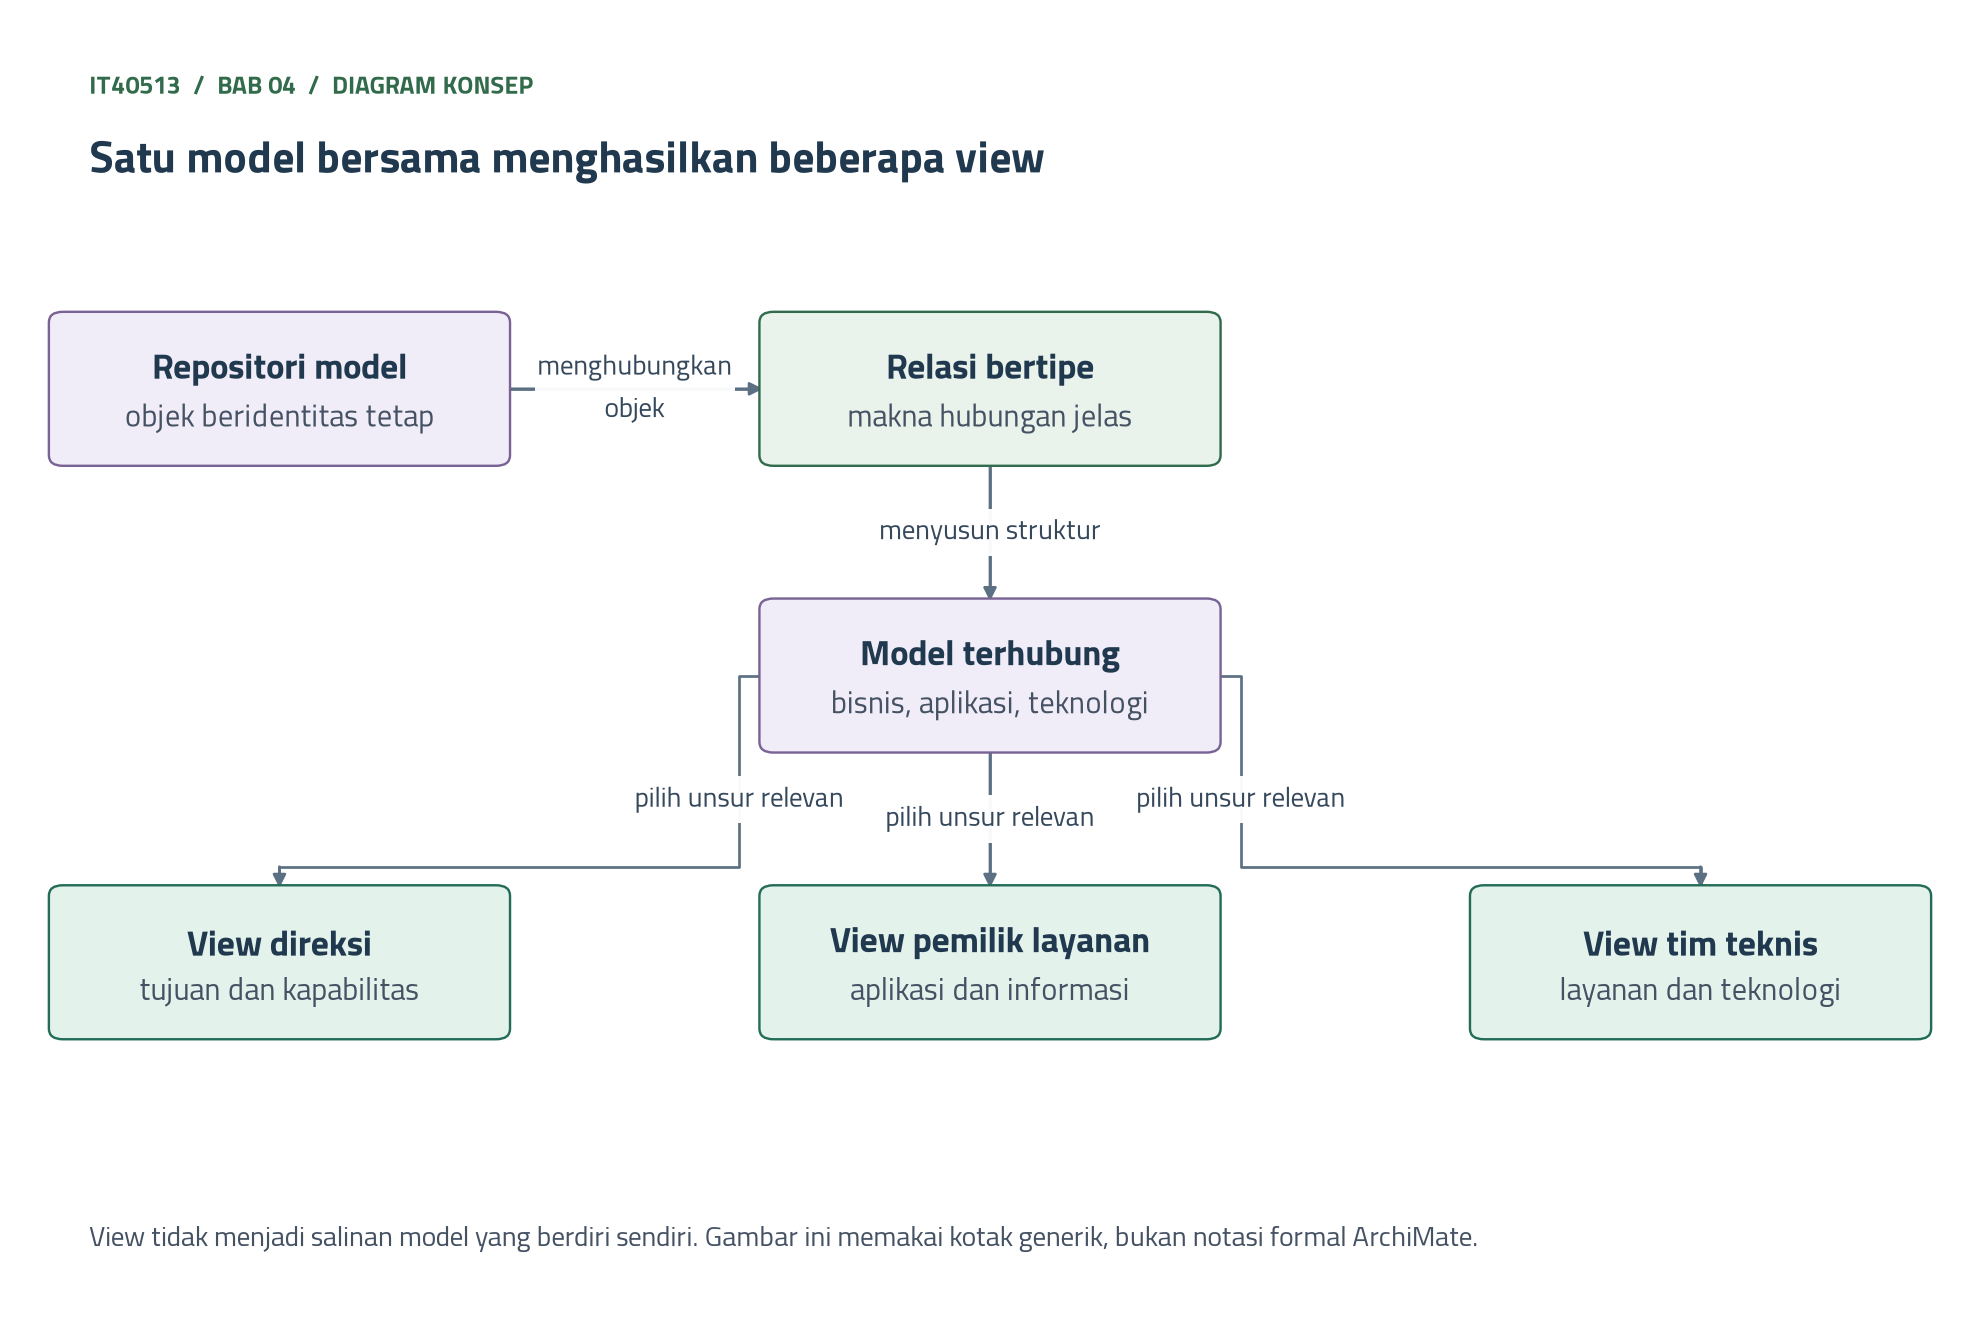
\includegraphics[width=0.96\textwidth,height=0.77\textheight,keepaspectratio]{../../figures/ch04-diagram-konsep.png}
  \label{fig:session04-ilustrasi-bab}
\end{frame}

\begin{frame}{{\Large Empat Viewpoint Paling Sering Dipakai}}
  \scriptsize
  \begin{tabularx}{\textwidth}{>{\raggedright\arraybackslash}p{2.4cm}
      >{\raggedright\arraybackslash}X >{\raggedright\arraybackslash}p{2.8cm}
      >{\raggedright\arraybackslash}X}
    \hline
    \textbf{\textit{Viewpoint}} & \textbf{Pertanyaan yang dijawab} & \textbf{Pembaca utama} & \textbf{Yang sengaja tidak tampil} \\
    \hline
    \textit{Layered} & Bagaimana satu layanan ditopang aplikasi dan teknologi dari ujung ke ujung? & Arsitek, kepala TI & Rantai motivasi, rincian langkah proses \\
    \hline
    \textit{Motivation} & Mengapa perubahan ini dilakukan, dan apa ukuran berhasilnya? & Direksi, pemilik program & Aplikasi dan teknologi \\
    \hline
    \textit{Application cooperation} & Aplikasi mana bertukar data dengan aplikasi mana? & Tim integrasi, analis teknologi & Proses bisnis, server \\
    \hline
    \textit{Capability map} & Apa saja yang mampu dilakukan organisasi? & Direksi, perencana strategi & Proses, aplikasi, unit organisasi \\
    \hline
  \end{tabularx}
\end{frame}

\begin{frame}{{\Large Dua View dari Satu Model}}
  \centering
  \eadiagram{../../figures/ch04-dua-view.tex}
\end{frame}

\begin{frame}{{\Large Kasus: Direksi dan Tim TI}}
  \begin{block}{Kasus Medikara Health}
    \small
    \begin{itemize}
      \item Rapat direksi bertanya aplikasi mana yang menopang layanan pasien dan di mana risikonya.
      \item Rapat tim TI bertanya bagaimana Medikara+ tersambung ke kelima SIMRS.
      \item \textit{View} direksi: tiga layanan bisnis dan dua aplikasi. Kelima SIMRS diringkas menjadi
            satu kotak merah ``5 versi berbeda''.
      \item \textit{View} tim TI: layanan bisnis dibuang, SIMRS dipecah menjadi lima komponen aplikasi.
      \item Lima garis memperlihatkan lima integrasi \textit{point-to-point}, bahan biaya di Bab 7.
    \end{itemize}
  \end{block}
\end{frame}

\section{Archi dan Aktivitas}

\begin{frame}{\hfill}
  \centering
  \Huge{\textbf{Archi dan Aktivitas}}
\end{frame}

\begin{frame}{{\Large Bekerja dengan Archi}}
  \small
  \begin{itemize}
    \item Archi 5.10.0 gratis dan bersumber terbuka. Satu berkas \texttt{.archimate} menyimpan seluruh
          elemen, relasi, dan \textit{view}.
    \item Elemen disimpan di folder tetap sesuai jenisnya. Subfolder boleh dibuat.
    \item Empat properti: Pemilik, Status, Sumber, dan Lokasi untuk \textit{node}.
    \item Ekspor: gambar, laporan HTML, berkas CSV, atau Open Exchange Format. Validator memeriksa model
          sebelum dibagikan.
    \item Kerja bersama: pemodel memegang berkas induk, atau \textit{plug-in} coArchi dengan repositori
          Git. Pilihan kedua mencatat riwayat, tetapi anggota harus belajar dasar Git.
  \end{itemize}
\end{frame}

\begin{frame}{{\Large Konvensi Penamaan Elemen}}
  \scriptsize
  \begin{tabularx}{\textwidth}{>{\raggedright\arraybackslash}p{2.4cm}
      >{\raggedright\arraybackslash}X >{\raggedright\arraybackslash}p{3.4cm}
      >{\raggedright\arraybackslash}p{2.2cm}}
    \hline
    \textbf{Jenis elemen} & \textbf{Pola nama} & \textbf{Contoh benar} & \textbf{Dihindari} \\
    \hline
    Proses & Kata kerja dan objeknya & Membuat Janji Temu & Proses Janji Temu \\
    \hline
    Fungsi & Kata benda berimbuhan pe-an & Pengelolaan Jadwal Dokter & Kelola Jadwal \\
    \hline
    Layanan & Kata ``Layanan'' dan hasil yang diterima pemakai & Layanan Pemesanan Jadwal & API Jadwal v2 \\
    \hline
    Komponen aplikasi & Nama yang dipakai pengguna, ditambah lokasi bila versinya berbeda & SIMRS RS Jakarta & HIS Bekasi \\
    \hline
    Peran & Nama peran, bukan nama orang & Petugas Pendaftaran & Bu Rina \\
    \hline
    Objek data & Kata benda tunggal dalam bahasa bisnis & Data Jadwal Dokter & tbl\_jadwal \\
    \hline
    \textit{View} & Jenis \textit{view}, titik dua, dan topiknya & Layered View: Janji Temu Rawat Jalan & Default View \\
    \hline
  \end{tabularx}
\end{frame}

\begin{frame}{{\Large Dari ArchiMate 3.2 ke ArchiMate 4}}
  \scriptsize
  \begin{tabularx}{\textwidth}{>{\raggedright\arraybackslash}p{3.8cm}
      >{\raggedright\arraybackslash}p{3.2cm} >{\raggedright\arraybackslash}X}
    \hline
    \textbf{ArchiMate 3.2} & \textbf{ArchiMate 4} & \textbf{Dampak pada model Medikara} \\
    \hline
    Lapisan bisnis, aplikasi, teknologi & Domain & Istilah berubah, susunan \textit{view} tetap \\
    \hline
    Proses, fungsi, layanan, dan peristiwa per lapisan & Satu set elemen perilaku umum & Layanan bisnis dan layanan aplikasi menjadi satu jenis \\
    \hline
    Peran bisnis & Peran umum & Peran dapat dipasang pada komponen aplikasi atau \textit{node} \\
    \hline
    Kolaborasi per lapisan & Satu elemen kolaborasi & Kolaborasi antarrumah sakit dan antaraplikasi memakai elemen yang sama \\
    \hline
    Relasi tanpa jumlah & Relasi dengan multiplisitas & ``Satu pasien punya banyak janji temu'' dapat dinyatakan di model \\
    \hline
    Interaksi, \textit{constraint}, kontrak, \textit{gap}, representasi & Dihapus & Elemen \textit{gap} yang dipakai di Bab 11 perlu dicatat dengan cara lain \\
    \hline
  \end{tabularx}

  \vspace{6pt}
  \small The Open Group menerbitkan ArchiMate 4 (dokumen C260) pada 27 April 2026.
\end{frame}

\begin{frame}{{\Large Mengapa Tetap ArchiMate 3.2}}
  \vspace{6pt}
  \small
  \begin{itemize}
    \item Archi 5.10.0 masih mendukung ArchiMate 3.2 dan belum mendukung ArchiMate 4.
    \item Open Exchange Format yang berlaku disusun untuk ArchiMate 3.1 dan 3.2.
    \item Berganti versi di tengah semester menambah risiko tanpa menambah nilai bagi pembaca.
    \item Persiapan pindah: interaksi tidak dipakai. \textit{Constraint} diganti \textit{requirement},
          dan kontrak diganti objek bisnis, keduanya diberi properti.
    \item Nama layanan dan proses menyiratkan domainnya. Jumlah yang penting ditulis di dokumentasi
          relasi.
  \end{itemize}
\end{frame}

\begin{frame}{{\Large Aktivitas: Peran dan Langkah}}
  \vspace{6pt}
  \small
  \begin{itemize}
    \item Analis bisnis memodelkan lapisan bisnis. Analis teknologi memodelkan lapisan aplikasi dan
          teknologi.
    \item Pemodel menyiapkan berkas, folder, dan konvensi. Koordinator memindahkan rantai motivasi C1 ke
          \textit{motivation view}.
    \item Pasang Archi 5.10.0, buka model contoh, pilih satu layanan inti, lalu tulis batasnya.
    \item Isi elemen tiap lapisan, sepakati titik sambung, lalu susun \textit{layered view}.
    \item Periksa nama dengan glosarium C1, jalankan Validator, lalu ekspor laporan HTML.
  \end{itemize}
\end{frame}

\begin{frame}{{\Large Luaran C2 dan Kriteria Penilaian}}
  \footnotesize
  \begin{tabularx}{\textwidth}{>{\raggedright\arraybackslash}p{4.0cm} r
      >{\raggedright\arraybackslash}X}
    \hline
    \textbf{Kriteria} & \textbf{Bobot} & \textbf{Tanda terpenuhi} \\
    \hline
    Kelengkapan rantai & 30\% & Rantai tidak putus dari penerima layanan sampai \textit{node} \\
    \hline
    Ketepatan relasi & 25\% & Arah melayani benar, asosiasi hanya dipakai bila tidak ada relasi lain yang cocok \\
    \hline
    Keterbacaan \textit{view} & 20\% & Paling banyak 20 elemen per \textit{view}, tata letak per lapisan \\
    \hline
    Keterlacakan ke C1 & 15\% & Minimal satu \textit{requirement} terhubung ke elemen inti \\
    \hline
    Konsistensi nama & 10\% & Nama sama dengan glosarium C1 dan mengikuti konvensi \\
    \hline
  \end{tabularx}

  \vspace{6pt}
  \small Luaran: model awal dengan satu \textit{layered view}, satu \textit{motivation view}, dan laporan
  HTML. Model tidak memuat data pribadi. Berkas: \berkas{sources/chapter04/README.md}.
\end{frame}

\begin{frame}{{\Large Ringkasan}}
  \vspace{6pt}
  \small
  \begin{itemize}
    \item Model menyimpan arti di elemen dan relasi. \textit{View} menampilkan sebagian isinya untuk
          pembaca tertentu.
    \item Kerangka inti: tiga lapisan kali tiga aspek, disambung lewat layanan.
    \item Relasi memberi arti pada garis. Aturan penurunan meringkas rantai panjang.
    \item \textit{Viewpoint} menentukan apa yang boleh tampil untuk menjawab satu \textit{concern}.
    \item Pesan utama: cetak biru yang dapat dipercaya dibangun dari satu model bersama, bukan dari
          kumpulan gambar, dan setiap gambar menjawab pertanyaan seorang pembaca tertentu.
  \end{itemize}
\end{frame}

\begin{frame}{{\Large Latihan}}
  \vspace{6pt}
  \small
  \begin{enumerate}
    \item Rantai Elemen untuk Layanan Pendaftaran: telusuri layanan pendaftaran pasien rawat jalan dari
          pasien sampai server basis data SIMRS. Tulis jenis elemen dan relasi tiap langkah.
    \item Memilih Viewpoint untuk Direktur: \textit{concern}-nya aplikasi mana yang mendukung tiap layanan
          pasien. Pilih \textit{viewpoint}, buat \textit{view}, lalu bandingkan jumlah elemennya dengan
          16 elemen \textit{layered view}.
    \item Menghitung Dampak ArchiMate 4: hitung jumlah dan persentase elemen model yang terdampak. Pada
          model contoh Medikara, hasilnya 10 dari 26 elemen, atau 38 persen.
  \end{enumerate}
\end{frame}

\begin{frame}{{\Large Bacaan dan Berkas Pendukung}}
  \vspace{10pt}
  \begin{itemize}
    \item \href{https://publications.opengroup.org/standards/archimate/c226}{\textit{ArchiMate 3.2 Specification}}
    \item \href{https://www.archimatetool.com/download/}{\textit{Archi: Open Source ArchiMate Modelling Tool}, Versi 5.10.0}
    \item \href{https://www.iso.org/standard/74393.html}{\textit{Software, Systems and Enterprise: Architecture Description}}
    \item \berkas{sources/chapter04/README.md}
  \end{itemize}
\end{frame}

\end{document}
